% 2.6 =============== 新古典增长模型初步数值解法 ===============

\section{数值解法初步：值函数迭代}  \label{sec-numerical-methods-pre}

在大多数情形下，我们都无法得到动态规划问题的解析解，只能对其进行逼近。
整体层面看，求解思路可以分为全局解和局部解：前者主要基于数值逼近，后者主要基于稳态附近的泰勒展开。
局部算法虽然速度较快，但其准确度和适用范围相对欠缺，例如当经济偏离稳态或受到较大冲击是，局部算法可能不再有效。
因此我们将先把精力集中于数值方法或者说全局算法。

事实上，模型解法的分类是多样的，更细致层面看，全局算法也可分为基于值函数和策略函数的方法。
本节将先介绍最基本的\textbf{值函数迭代方法}（Value Function Iteration，VFI）及其改进，这是由压缩映射定理保证的；
在下一节，我们将\textbf{进一步基于策略函数（欧拉方程）}来求解RCK模型；
最后，本章将介绍\textbf{投影法}（Projection）中\textbf{配置算法}（Collocation Method）的实现
（事实上VFI本身就是一种特殊的投影法）。


% 2.6.1 ===== VFI =====
\subsection{值函数迭代基本算法}

考虑如下一般形式的优化问题：个体通过决定控制变量的路径$\{y_t\}_{t=0}^{\infty}$来最大化其未来回报$u(y_t,x_t)$之和，
\begin{equation*}
    v\left(x_t\right) = \max _{\left\{y_{t+s} \in \mathbb{D}\left(x_{t+s}\right)\right\}_{s=0}^{\infty}} 
        \sum_{s=0}^{\infty} \beta^s u\left(y_{t+s}, x_{t+s}\right)
\end{equation*}
其中，$\beta$是折现因子，$\mathbb{D}(\cdot)$是控制变量的可行集，$x_t$是控制变量且运动方程满足：
\begin{equation*}
    x_{t+1} = h(x_t,y_t), ~x_0\text{给定}
\end{equation*}
我们已经知道如何将这一问题转化为动态规划形式，并可得到一般化的贝尔曼方程：
\begin{equation}
    v(x) = \max_{y\in\mathbb{D}(x)} u(y,x) + \beta v(x^{\prime})
\end{equation}
以及对应的决策规则（策略函数）：
\begin{equation*}
    y = g(x) = \underset{y \in \mathbb{D}(x)}{\operatorname{argmax}}~u(y,x)+\beta v(x^{\prime})
\end{equation*}
我们的目标是从Bellman方程中解出值函数$v$。
在此前，我们以连续逼近法作为引例，证明了值函数的存在与唯一性，并构造了找到贝尔算子不动点的一个算法。
简单回忆这一构造流程：

\textbf{Step 1.} 任意挑选一个初始值函数$v^0(x)$作为猜测，例如$v^0(x) = 0,~ \forall x$

\textbf{Step 2.} \textbf{构造单调递增的值函数序列}：对所有$x$，定义：
\begin{equation*}
    v^{n+1}\left(x\right) = \max _{y\in\mathbb{D}(x)}
        \left[u\left(y,x\right)+\beta v^n\left(x^{\prime}\right)\right],\quad n = 0,1,\dots
\end{equation*}

我们已经证明了值函数序列$\{v^n(x)\}$是单调递增的，即$v^{n+1} = Tv^n \geq v^n$；
并且利用\textbf{压缩映射定理}证明了不动点$v=Tv$的存在性，进而也就从算法层面证明了上述步骤最终会收敛。
\footnote{Blackwell充分条件对单调性做出了要求，这是构造单例序列的原因。}
用数学语言表述的话，计算贝尔曼方程解的直观方法是\textbf{迭代算子$T$直至$v^{n+1}$和$v^n$距离足够小}。
具体而言，迭代所得的序列满足：
\begin{itemize}
    \item $\{v^j(x)\}_{j=0}^{\infty}$收敛至动态规划问题的真实解$v(x)$；
    \item 值函数序列与真实解$v(x)$的距离以一个常数速率越来越小：$\|v^{n+1}-v\| \leq \beta \|v^{n}-v\|$。
\end{itemize}

在实践中，计算机并不能存储连续的（无限维）函数，因此要\textbf{先对连续的状态变量空间等进行离散化}（Dicretation）。
下方给出了利用\textbf{值函数迭代}求解贝尔曼方程的基本算法：

\begin{mdframed}[linecolor=Black,linewidth=1pt]
    \textbf{算法：值函数迭代}

    \textbf{输入：}模型参数（折现率、折旧率、风险偏好等）；算法参数（格点维数、停止准则等）

    \textbf{输出：}值函数$v$和策略函数$g$

    \textbf{1. 初始化：}

    将状态变量$x$的取值空间离散化为格点：
    \begin{equation*}
        \mathbb{X} = \{x_1<x_2<\cdots<x_i<\cdots<x_N\}
    \end{equation*}
    设定迭代次数$iter=0$，猜测初始值函数向量$v^0(x)$
    \begin{equation*}
        \left[v^0(x_1),v^0(x_2),\cdots,v^0(x_i),\cdots,v^0(x_N)\right]^{\prime}
    \end{equation*}
    选择停止准则$\varepsilon>0$

    \textbf{2. 求解贝尔曼方程右侧：}

    对任意$x_{i}\in\mathbb{X},~ i=1,\cdots,x_N$，计算最大化后（迭代后）的值函数：

    \begin{equation*}
        v^{iter+1}(x_i) \equiv v^{iter+1}_i = \max_{x^{\prime}} u\left(y\left(x_i,x^{\prime}\right),x_i\right)
            + \beta v^{iter}(x^{\prime})
    \end{equation*}
    记录并更新与之对应的策略函数：
    \begin{equation*}
        g(x_i) \equiv g_i = \underset{j}{\operatorname{argmax}}
            u\left(y\left(x_i,x^{\prime}\right),x_i\right) + \beta v^{iter}(x^{\prime})
    \end{equation*}

    \textbf{3. 检验停止准则：}

    若$\left\|v^{iter+1}(x)-v^{iter}(x)\right\|<\varepsilon$，则进行停止迭代，输出值函数和策略函数；
    否则回到第2步。
\end{mdframed}

由于贝尔曼算子是压缩映射，上述过程一定会收敛。同时，我们可以记录下了与$x_i$相对应的最优的$y=g(x_i)$，进而也就得到了策略函数。
我们称上述过程为\textbf{值函数迭代}。为了加深理解，下方给出一个确定性RCK模型的示例及相应代码。

\begin{example}
    \textbf{值函数迭代求解RCK：}假设效用函数形式为：
    \begin{equation*}
        u(c) = \frac{c^{1-\sigma}-1}{1-\sigma}
    \end{equation*}
    资本积累方程为：
    \begin{equation*}
        k^{\prime} = f(k) - c + (1-\delta)k = k^{\alpha} - c + (1-\delta)k
    \end{equation*}
    由消费和资本的非负性，贝尔曼方程为：
    \begin{equation*}
        \begin{aligned}
            v(k) &= \max _{0 \leq c \leq k^\alpha+(1-\delta) k} 
                \frac{c^{1-\sigma}-1}{1-\sigma}+\beta v\left(k^{\prime}\right) \\
            &= \max_{0\leq k^{\prime} \leq k^\alpha+(1-\delta) k}
                \frac{\left(k^\alpha+(1-\delta) k-k^{\prime}\right)^{1-\sigma}-1}{1-\sigma}+\beta v\left(k^{\prime}\right)
        \end{aligned}
    \end{equation*}
    我们希望求解出值函数和策略函数。

    首先，将资本$k$的取值空间离散化为$n_k$维格点：
    \begin{equation*}
        \mathbb{K}=\left\{k_1 < \cdots < k_{n_k}\right\}
    \end{equation*}
    设定迭代次数$iter=0$，猜测在这些格点上取值的$n_k$维初始值函数向量：
    \begin{equation*}
        v^0(k) = \left[v^0_1=v^0_{k_{1}},v^0_2,\cdots,v^0_i=v^0(k_i),\cdots,v^0_n=v^0_{k_{n_k}}\right]^{\prime}
    \end{equation*}
    选择算法的停止准则$\varepsilon>0$。

    接着，对每一个$i=1\cdots,n_k$，计算当前第$iter$次迭代中可行$j$下的：
    \begin{equation*}
        v_{ij} \equiv \frac{\left(k_i^{\alpha}+\left(1-\delta\right)k_i-k_j\right)^{1-\sigma}-1}{1-\sigma} + 
            \beta v^{iter}(k_j)
    \end{equation*}
    这里要\textbf{特别注意可行$j$的概念}：消费的非负性和最大值对下期资本可行集的范围做出了限制，即：
    \begin{equation*}
        0\leq k^{\prime} \leq k^{\alpha}+(1-\delta)k
    \end{equation*}
    进而限定了下期资本\textbf{可选的脚标$j$下界和上界。}
    就下界而言，可以通过选择合适的格点$k_1$使得$\underbar{j}=1$；
    就上界而言，假设取值格点是均匀分布的，即
    \begin{equation*}
        k_h=k_1+(h-1)d_k,~h=1,\cdots,n_k
    \end{equation*}
    其中$d_k$是间隔，从而对任意当前格点$k_i$，可以由上式和资本取值范围计算与之对应的下期资本脚标$j$的上界
    （由于格点递增，这相当于给定当前$k_i$，找到保证消费非负的最大下期资本的取值）：
    \begin{equation*}
        \begin{aligned}
            k_j\equiv k_1+(j-1)d_k \leq k_i^{\alpha}+(1-\delta)k_i \\
            \Leftrightarrow \\
            j \leq \frac{k_i^{\alpha}+(1-\delta)-k_1}{d_k} + 1
        \end{aligned}
    \end{equation*}
    由于格点脚标是正整数并且最大为$n_k$，因此有：
    \begin{equation*}
        \bar{j} = \min \{floor({\frac{k_i^{\alpha}+(1-\delta)k_i-k_{1}}{d_k}})+1,n_k\}
    \end{equation*}
    从而可以得到：
    \begin{equation*}
        v_{ij}^* = \max_{j=1,\cdots,\bar{j}} v_{ij} = \max_{j=1,\cdots,\bar{j}}
            \frac{\left(k_i^{\alpha}+\left(1-\delta\right)k_i-k_j\right)^{1-\sigma}-1}{1-\sigma} + 
                \beta v^{iter}(k_j)
    \end{equation*}
    即完成了任意给定当前资本存量$k_i$下的一次迭代，可设定：
    \begin{equation*}
        v^{iter+1}(k_i) = v_{ij}^*
    \end{equation*}
    并记录下对应的最优脚标$j^* = \operatorname{argmax}_{j=1,\cdots,\bar{j}}v_{ij}$，也即策略函数：
    \begin{equation*}
        k^{\prime}(k_i) = k_{j^*}
    \end{equation*}

    最后，计算误差，若$\left\|v^{iter+1}(k)-v^{iter}(k)\right\|<\varepsilon$，停止迭代；否则令迭代次数$iter+1$
    并返回上一步。直至收敛。下面给出了对应的Matlab代码。
\end{example}

\begin{lstlisting}
    clear;clc;
    %% setup
    % economic parpam
    alpha = 0.3;
    sigma = 1.5;
    beta = 0.95;
    delta = 0.1;

    ks = ((1-beta*(1-delta)) / (alpha*beta))^(1/(alpha-1));
    csy	= 1-alpha*beta*delta/(1-beta*(1-delta));

    % numerical param
    nk = 1000;
    epsilon = 1e-6;
    dev = 0.9;

    % discretize k
    kmin = (1-dev)*ks;
    kmax = (1+dev)*ks;
    dk = (kmax-kmin)/(nk-1);
    kgrid = linspace(kmin,kmax,nk)';

    %% iteration on bellman operator
    % initialize
    error = 1;
    %v = zeros(nk,1);    % value function
    v = ((csy*kgrid.^alpha).^(1-sigma)-1)./((1-sigma)*(1-beta));
    tv = zeros(nk,1);
    g = zeros(nk,1);   % decision rule: index
    iter = 1;

    % iteration
    tic
    while error > epsilon
    for i = 1:nk
        % compute min index for next period k
        jmin = max(ceil(((1-delta)*kgrid(i)-kmin)/dk)+1,1);
        % compute max index for next period k because consumption>0
        tmp = kgrid(i)^alpha + (1-delta)*kgrid(i) - kmin; 
        jmax = min(floor(tmp/dk)+1, nk);
        
        % all possible to be compared: (jmax-jmin)*1 dimension
        c = kgrid(i)^alpha + (1-delta)*kgrid(i) - kgrid(jmin:jmax); 
        u = (c.^(1-sigma)-1) / (1-sigma); 
        
        % bellman operator：用itemp是因为v的index从1而不是jmin开始
        [tv(i),jtmp] = max(u + beta*v(jmin:jmax));
        g(i) = jmin-1+jtmp;
    end
    error = max(abs(tv-v));
    v = tv;
    iter = iter + 1;
    end
    toc

    %% solution
    kprime = kgrid(g);  % policy function
    c = kgrid.^alpha + (1-delta)*kgrid - kprime;
\end{lstlisting}

在上述代码中，设定了取$n_k = 1000$个格点来代表资本$k$的取值空间，设定对稳态上下偏离90\%作为格点的最大和最小值，
用时4.8秒。\cref{fig-vfirck-value-policy-func}绘制了由VFI得到的值函数和策略函数，它具备前文所证明的相关性质。
\begin{figure}[H]
    \centering
    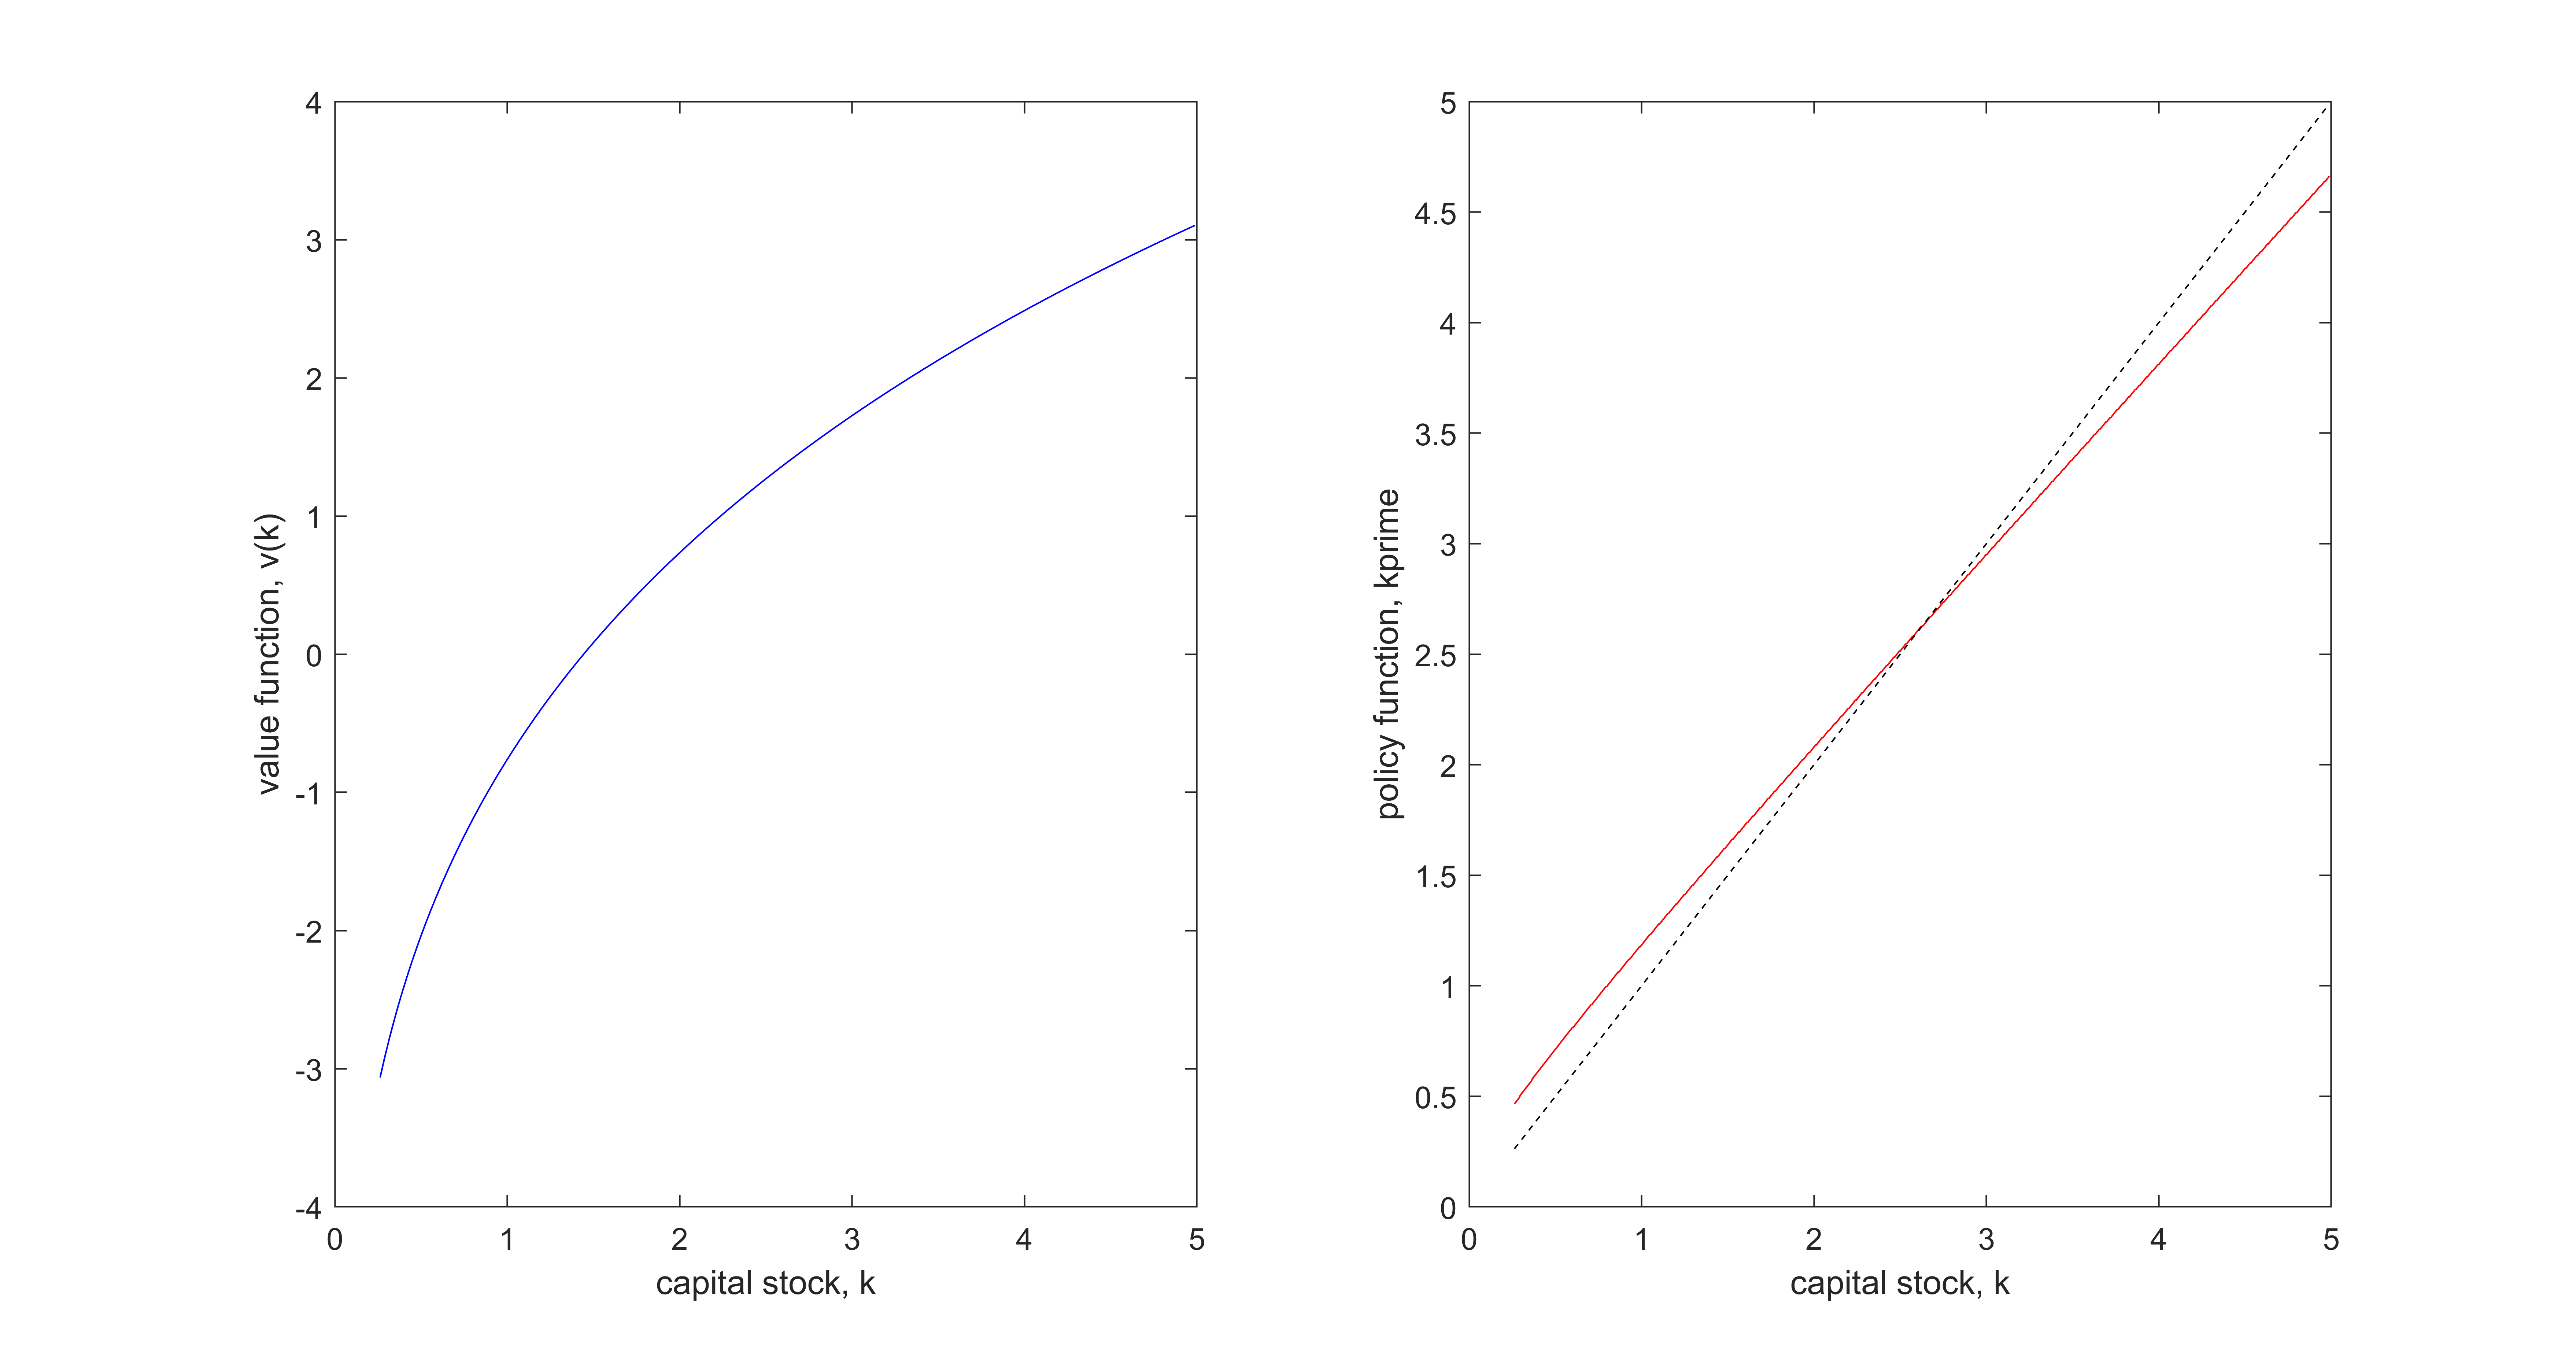
\includegraphics[width=1\textwidth]{figures/part1/ch2/fig-vfirck-value-policy-func.png}
    \caption{值函数与策略函数}
    \label{fig-vfirck-value-policy-func}
\end{figure}

% 2.6.2 ===== 改进VFI =====
\subsection{改进值函数迭代：插值}

上述方法的潜在问题之一是：\textbf{真实下期最优资本存量未必在我们设定的格点上}，
我们也就无法得到值函数在这些实际位置的取值。一个改进思路是利用插值法对值函数进行估计。
将状态变量格点取得相对宽松，而将控制变量格点取得较为精细，这样可减少对函数的估计次数，从而降低运算时间。
对如下形式的贝尔曼方程：
\begin{equation*}
    v(x) = \max_{y\in\mathbb{D}(x)} u(y,x) + \beta v(x^{\prime})
\end{equation*}
改进算法如下：

\begin{mdframed}[linecolor=Black,linewidth=1pt]
    \textbf{算法：改进值函数迭代}

    \textbf{输入：}模型参数（折现率、折旧率、风险偏好等）；算法参数（格点维数、停止准则等）

    \textbf{输出：}值函数$v$和策略函数$g$

    \textbf{1. 离散化状态变量和控制变量：}

    将状态变量$x$的取值空间离散化为较宽松的$N$个格点：
    \begin{equation*}
        \mathbb{X} = \{x_1<x_2<\cdots<x_i<\cdots<x_N\}
    \end{equation*}
    将控制变量$y$的取值空间离散化为较为精细的$M$个格点：
    \begin{equation*}
        \mathbb{Y} = \{y_1<y_2<\cdots<y_i<\cdots<y_M\}, ~ M \gg N
    \end{equation*}
    设定迭代次数$iter=0$，猜测初始值函数向量$v^0(x)$
    \begin{equation*}
        \left[v^0(x_1),v^0(x_2),\cdots,v^0(x_i),\cdots,v^0(x_N)\right]^{\prime}
    \end{equation*}
    选择停止准则$\varepsilon>0$

    \textbf{2. 求解贝尔曼方程右侧：}

    对任意$x_{i}\in\mathbb{X},~ i=1,\cdots,x_N$，根据运动方程计算下期状态：
    \begin{equation*}
        x^{\prime}_{ij} = h(y_j,x_i), ~\forall j=1,\cdots,M
    \end{equation*}
    \textbf{利用插值方法计算值函数在$x^{\prime}_{ij}=h(y_j,x_l)$处，当前迭代下的值函数取值}$\tilde{v}^{iter}(x^{\prime}_{ij})$，
    据此求解贝尔曼方程右侧：
    \begin{equation*}
        v^{iter+1}(x_i) \equiv v^{iter+1}_i = \max_{y\in\mathbb{Y}} u\left(y,x_i\right)
            + \beta \tilde{v}^{iter}(x^{\prime}_{ij})
    \end{equation*}

    \textbf{3. 检验停止准则：}

    若$\left\|v^{iter+1}(x)-v^{iter}(x)\right\|<\varepsilon$，则进行停止迭代，输出值函数和策略函数；
    否则回到第2步。
\end{mdframed}

\begin{lstlisting}
    %% setup
    % economic parpam
    alpha = 0.3;
    sigma = 1.5;
    beta = 0.95;
    delta = 0.1;

    ks = ((1-beta*(1-delta)) / (alpha*beta))^(1/(alpha-1));
    csy	= 1-alpha*beta*delta/(1-beta*(1-delta));

    % numerical param
    nk = 20;
    nc = 1000;
    epsilon = 1e-6;
    dev = 0.9;

    % discretize k
    kmin = (1-dev)*ks;
    kmax = (1+dev)*ks;
    kgrid = linspace(kmin,kmax,nk)';

    % discretize c
    cmin = 0.01;
    cmax = kmax^alpha;
    cgrid = linspace(cmin,cmax,nc)';

    %% iteration on bellman operator
    % initialize
    error = 1;
    v = ((csy*kgrid.^alpha).^(1-sigma)-1)./(1-sigma);    % value function
    tv = zeros(nk,1);
    g = zeros(nk,1);   % decision rule: index
    u = (cgrid.^(1-sigma)-1) / (1-sigma);
    iter = 1;

    % iteration
    tic
    while error > epsilon
    for i = 1:nk
        % all possible kp when ki now: nc*1 dimension
        kp = kgrid(i).^alpha + (1-delta)*kgrid(i) - cgrid; 
        % interp one函数用于正在kp处插值：nc*1 dimension
        vinterpl = interp1(kgrid,v, kp, 'spline'); 
        
        % bellman operator
        [tv(i),g(i)] = max(u+beta*vinterpl);
    end
    error = max(abs(tv-v));
    v = tv;
    iter = iter + 1;
    end
    toc

    %% solution
    c = cgrid(g);
    % kprime = kgrid(g);
    kprime = kgrid.^alpha+(1-delta)*kgrid-c;
\end{lstlisting}

用时仅0.05秒。


% =====   =====
\subsection{值函数迭代的改进：}



% =====   =====
\subsection{投影法的初步实现：配置算法}



% =====   =====
\subsection{Euler Based Methods}



